\section{The fragments $\AAbarBBbar$ and $\AAbarEEbar$}\label{sec:AAbarEEbar}
In this section, we show that the MC problem for the fragments $\AAbarBBbar$ and $\AAbarEEbar$  is \PSPACE-complete.
Moreover, we prove that MC for the smaller fragments $\B$ and $\E$ is $\co\NP$-complete.

\subsection{Polynomial small-model property for $\AAbarBBbar$ and $\AAbarEEbar$}\label{subsec:polyAAbarEEbar}
We first prove membership to \PSPACE\ of the MC problem for the fragments $\AAbarBBbar$ and $\AAbarEEbar$ by showing that they feature a \emph{polynomial small-model property}, that is, we prove that if a trace $\rho$ of a finite Kripke structure $\Ku$ satisfies a given formula $\varphi$ of $\AAbarEEbar$ or $\AAbarBBbar$, then there exists a trace $\pi$, whose length is polynomial in the sizes of $\varphi$ and $\Ku$, starting from, and leading to, the same states as $\rho$, that satisfies $\varphi$. In the following, we focus on $\AAbarEEbar$, being the case of $\AAbarBBbar$ completely symmetric.

Let $\Ku= \KuDef$ be a finite Kripke structure.
We start by introducing the basic notions of \emph{induced trace} and \emph{well-formed trace}, that will be extensively used to prove the polynomial small-model property. 
%
Intuitively, we say that a trace $\pi\in\Trk_{\Ku}$ is induced by a trace $\rho\in\Trk_{\Ku}$ if it can be obtained from 
$\rho$ by suitably contracting it, that is, by concatenating some subtraces of $\rho$.
%, provided that the resulting sequence is a trace of $\Ku$ as well. 
Well-formedness adds a condition on the suffixes of an induced trace.
For the sake of readability, hereafter we denote by $\rho^i$ the suffix $\rho(i,|\rho|)$ of $\rho$ (hence, $\rho^1$ is just $\rho$).

\begin{definition}[Induced and well-formed trace] \label{definition:inducedTrk}
Let $\Ku\!=\! \KuDef$ be a finite Kripke structure and let $\rho\in\Trk_\Ku$, with $|\rho| = n$. 
A trace $\pi\in\Trk_\Ku$ is \emph{induced} by $\rho$ if there exists an increasing sequence of 
$\rho$-positions $i_1<\ldots < i_k$, with $i_1=1$ and $i_k=n$, such that $\pi= \rho(i_1)\cdots \rho(i_k)$.
For $j = 1, \ldots, k$, the $\pi$-position $j$ and the $\rho$-position $i_j$ are called \emph{corresponding positions}.

An induced trace $\pi$ is \emph{well-formed} (with respect to $\rho$) if, for all $\pi$-positions $j$, with corresponding $\rho$-positions $i_j$, and all proposition letters $p\in \Prop$, it holds that
\[\Ku,\pi^{j} \models p \iff \Ku,\rho^{i_j} \models p.\]
\end{definition}

\begin{example}
As an example, let us consider Figure~\ref{fig:induced}. The trace $\pi = \rho(1)\rho(4)\rho(5)\rho(7)\rho(10)$ is induced by $\rho$, provided that both $\rho$ and $\pi$ are traces of a Kripke structure $\Ku$, and the positions $1, 2, 3, 4$, and $5$ of $\pi$ correspond to the positions $i_1=1$, $i_2=4$, $i_3=5$, $i_4=7$ and $i_5=10$ of $\rho$.

\begin{figure}[H]
    \centering
    \resizebox{\linewidth}{!}{\includegraphics{Chaps/TCS17/induced}}
    %\vspace{-0.3cm}
    \caption{A trace $\pi$ induced by $\rho$.
    }
    \label{fig:induced}
\end{figure}
\end{example}

Note that if $\pi$ is induced by $\rho$, then $\fst(\pi)=\fst(\rho)$, $\lst(\pi)=\lst(\rho)$, and $|\pi|\leq |\rho|$ ($|\pi| = |\rho|$ if and only if $\pi = \rho$). 

Well-formedness implies that the suffix of $\pi$ starting from position $j$ and that of $\rho$ starting from the corresponding position $i_j$ agree over all the proposition letters in $\Prop$, that is, they have the same \lq\lq satisfaction pattern\rq\rq{} of proposition letters. In particular, for all $p\in \Prop$, $\Ku,\pi \models p$ if and only if $\Ku,\rho \models p$. It can be easily checked that the \emph{well-formedness relation is transitive}.

The following proposition shows how it is possible to contract a trace while preserving the same satisfaction pattern of proposition letters with respect to suffixes.  Such a criterion represents a ``basic step'' in a contraction process that will allow us to prove the polynomial small-model property. 

\begin{proposition}\label{proposition:wellFormdness}
Let $\Ku = \KuDef$ be a finite Kripke structure. For any trace $\rho\in\Trk_\Ku$, there exists a
well-formed (with respect to $\rho$) trace $\pi\in\Trk_\Ku$ such that $|\pi| \leq |\States|\cdot (|\Prop|+1)$.
\end{proposition}
\begin{proof}
Let $\rho\in\Trk_\Ku$, with $|\rho| = n$. If $n\leq |\States|\cdot (|\Prop|+1)$, the thesis trivially holds.
%
Let us assume $n > |\States|\cdot (|\Prop|+1)$. We show that there exists $\pi\in\Trk_\Ku$, with $|\pi| < n$, which is well-formed with respect to $\rho$.

Since $n> |\States|\cdot (|\Prop|+1)$, there is some state $s\in \States$ occurring in $\rho$ at least $|\Prop|+2$ times.
Assume that for all $\rho$-positions $i$ and $j$, with $j>i$, if $\rho(i)=\rho(j)=s$, then there exists some $p\in\Prop$ such that $\Ku,\rho^j \models p$ and $\Ku,\rho^i \not\models p$. This assumption leads to a contradiction, as the suffixes of $\rho$ may feature at most $|\Prop|+1$ distinct satisfaction patterns of proposition letters (due to the homogeneity assumption in Definition~\ref{def:inducedmodel}), while there are at least $|\Prop|+2$ occurrences of $s$.
As a consequence, there are two $\rho$-positions $i$ and $j$, with $j>i$, such that $\rho(i)=\rho(j)=s$ and, for all $p\in\Prop$, $\Ku,\rho^j \models p$ if and only if $\Ku,\rho^i \models p$ (see Figure~\ref{fig:basicContr} for a graphical account).
%
It is easy to see that $\pi=\rho(1, i)\star\rho(j, n)\in\Trk_\Ku$ is well-formed with respect to $\rho$ and $|\pi| < n$.  If $|\pi| \leq |\States|\cdot (|\Prop|+1)$, the thesis is proved; otherwise, the same basic step can be iterated a finite number of times, and the thesis follows by transitivity of the well-formedness relation.
\end{proof}


\begin{figure}[tb]
\centering
    \scalebox{1.8}{
    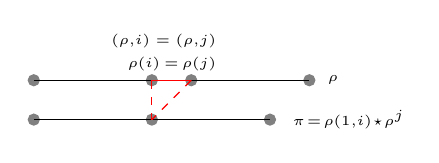
\begin{tikzpicture}
    				%				[->,>=stealth',shorten >=1pt,auto,node distance=0,main node/.style={circle,draw}]
    	\filldraw [gray] (0,0) circle (2pt)
    	(1.5,0) circle (2pt)
    	(2,0) circle (2pt)
    	(3.5,0) circle (2pt);
    	%
    	\filldraw [gray] (0,-0.5) circle (2pt)
    	(1.5,-0.5) circle (2pt)
    	(3,-0.5) circle (2pt);
    	%
    	\draw [red] (1.5,0) -- (2,0);
    	\draw [black]  (0,0) -- (1.5,0);
    	\draw [black] (2,0) -- (3.5,0);
    	\draw [black] (0,-0.5) -- (3,-0.5);
    	\draw [dashed, red] (1.5,0) -> (1.5,-0.5);
    	\draw [dashed, red] (2,0) -> (1.5,-0.5);
    	{\tiny
    		\node (a0) at (3.8,0) {$\rho$};	
    		\node (b0) at (4,-0.5) {$\pi\!=\!\rho(1,\! i)\!\star\! \rho^j$};	
    		\node (a1) at (1.4,0.2) {$\rho(i)$};
    		\node (a11) at (1.75,0.2) {$=$};
    		\node (a2) at (2.1,0.2) {$\rho(j)$};
    		\node (a3) at (1.65,0.5) {$\Prop(\rho,\! i)= \Prop(\rho,\! j)$};
    		%\node (a4) at (4.7,0.5) {$Pattern(\rho,k) =\{ p \in \Prop : \Ku,\rho^{k]} \models p\}$};
    			
    	}
    \end{tikzpicture}}
    \caption{The contraction step of Proposition~\ref{proposition:wellFormdness} ($\Prop(\rho,k)=\{ p \in \Prop \mid \Ku,\rho^{k} \models p\}$).}\label{fig:basicContr}
\end{figure}


The next definition identifies some distinguished positions in a trace, called \emph{witness positions}. As we will see in the proof of Theorem~\ref{theorem:polynomialSizeModelProperty}, if we perform a contraction (see the proof of Proposition~\ref{proposition:wellFormdness}, and its graphical account in Figure~\ref{fig:basicContr}) between a pair of such positions, we get a trace which is equivalent to the original one with respect to satisfiability of the considered $\AAbarEEbar$ formula. In the following, we restrict ourselves to formulas in \emph{negation normal form} (\nnf), namely, formulas where negation is applied only to proposition letters. By using De Morgan's laws and the dual modalities $\hsEu$, $\hsEtu$, $\hsAu$, and $\hsAtu$ of $\hsE$, $\hsEt$, $\hsA$, and $\hsAt$,  respectively, we can trivially convert (in linear time) a formula into an equivalent one in \nnf, having at most double length.

\begin{definition}[Witness position]\label{definition:WitnessPositions} 
Let $\Ku = \KuDef$ be a finite Kripke structure, $\rho\in\Trk_\Ku$, and $\varphi$ be a formula of $\AAbarEEbar$. Let us denote by $E(\varphi,\rho)$ the set of subformulas of the form $\hsE\psi$ of $\varphi$ such that $\Ku, \rho\models\hsE\psi$.

The \emph{set $Wt(\varphi,\rho)$ of witness positions of $\rho$ for $\varphi$} is the \emph{minimal} set of $\rho$-positions satisfying the following constraint:
\begin{itemize}
    \item for each $\hsE\psi\in E(\varphi,\rho)$, the greatest $\rho$-position $i>1$ such that $\Ku,\rho^i\models\psi$ belongs to $Wt(\varphi,\rho)$.\footnote{Note that such a $\rho$-position exists by definition of $E(\varphi,\rho)$.}
\end{itemize}
\end{definition}
It is easy to see that the cardinalities of $E(\varphi,\rho)$ and of $Wt(\varphi,\rho)$ are at most $|\varphi|-1$.
We are now ready to prove the polynomial small-model property.

\begin{theorem}[Polynomial small-model property for $\AAbarEEbar$]\label{theorem:polynomialSizeModelProperty}
Let $\Ku= \KuDef$ be a finite Kripke structure, $\rho, \sigma \in \Trk_\Ku$, and $\varphi$ be an $\AAbarEEbar$ formula in \nnf{} such that $\Ku,\rho\star\sigma\models \varphi$. Then there exists $\pi$, induced by $\rho$, such that $\Ku,\pi\star\sigma\models \varphi$, and $|\pi|\leq |\States|\cdot (|\varphi|+1)^2$.
\end{theorem}
%
As a preliminary remark, we note that the theorem holds in particular if $|\sigma|=1$, and thus $\rho\star\sigma=\rho$ and $\pi\star\sigma=\pi$. In such a case, if $\Ku,\rho\models \varphi$, then $\Ku,\pi\models \varphi$, where $\pi$ is induced by $\rho$ and $|\pi|\leq |\States|\cdot (|\varphi|+1)^2$. The more general statement of Theorem~\ref{theorem:polynomialSizeModelProperty} is needed for technical reasons in the soundness/completeness proofs of the  algorithms for MC given in the following.

\begin{proof}
W.l.o.g., we restrict ourselves to the proposition letters occurring in  $\varphi$, thus having $|\Prop|\leq |\varphi|$.
Let $Wt(\varphi,\rho\star\sigma)$ be the set of witness positions of $\rho\star\sigma$ for $\varphi$, let $\{i_1,\ldots,i_k\}$ be the ordering of $Wt(\varphi,\rho\star\sigma)$ such that $i_1<\ldots <i_k$, and let $i_0=1$ and $i_{k+1}=|\rho\star\sigma|$. Hence, $1=i_0< i_1<\ldots <i_k \leq i_{k+1}=|\rho\star\sigma|$.

If $|\rho| \leq |\States|\cdot (|\varphi|+1)^2$, the thesis trivially holds.
Let us assume that $|\rho|> |\States|\cdot (|\varphi|+1)^2$. We show that there exists a trace $\pi$ induced by $\rho$, with $|\pi| < |\rho |$, such that $\Ku,\pi\star\sigma\models \varphi$.

W.l.o.g., we can assume that, for some $j\geq 0$, $i_0<i_1<\ldots <i_j$ are $\rho$-positions, while $i_{j+1}<\ldots <i_{k+1}$ are $(\rho\star\sigma)$-positions not in $\rho$. 
%We claim that 
Then, either $(i)$ there exists $t\in [0,j-1]$ such that $i_{t+1}-i_t>|\States|\cdot(|\varphi|+1)$ or $(ii)$ $|\rho(i_j,|\rho|)|>|\States|\cdot(|\varphi|+1)$. By way of contradiction, suppose that neither $(i)$ nor $(ii)$ holds. We need to distinguish two cases. If $\rho\star\sigma=\rho$, then
$|\rho| = (i_{k+1}-i_0)+1\leq (k+1) \cdot |\States|\cdot (|\varphi|+1)+1$; otherwise ($|\rho| < |\rho\star\sigma|$), $|\rho| = (i_j - i_0) + |\rho(i_j,|\rho|)| \leq j \cdot |\States|\cdot (|\varphi|+1) + |\States|\cdot (|\varphi|+1) \leq (k+1) \cdot |\States|\cdot (|\varphi|+1)$. The contradiction follows since $(k+1) \cdot |\States|\cdot (|\varphi|+1)+1 \leq |\varphi| \cdot |\States|\cdot (|\varphi|+1)+1 \leq |\States|\cdot (|\varphi|+1)^2$.

Let 
%us define 
$(\alpha,\beta)=(i_t,i_{t+1})$ in case $(i)$, and $(\alpha,\beta)=(i_j,|\rho|)$ in case $(ii)$ and let $\rho'=\rho(\alpha,\beta)$. In both cases, 
%we have  
$|\rho'|> |\States|\cdot (|\varphi|+1)\geq |\States|\cdot (|\Prop|+1)$, being $|\Prop|\leq |\varphi|$.
%
By Proposition~\ref{proposition:wellFormdness}, there exists a trace $\pi'$ of $\Ku$, well-formed with respect to $\rho'$, such that $|\pi'|\leq |\States|\cdot(|\Prop|+1) < |\rho'|$. Let $\pi$ be the trace induced by $\rho$ obtained by replacing the subtrace $\rho'$ of $\rho$ by $\pi'$ (see Figure~\ref{fig:contr2} for a graphical account).
Since $|\pi|<|\rho|$, it remains to prove that  $\Ku,\pi\star\sigma\models \varphi$.

\begin{figure}[tb]
\centering
    \resizebox{\linewidth}{!}{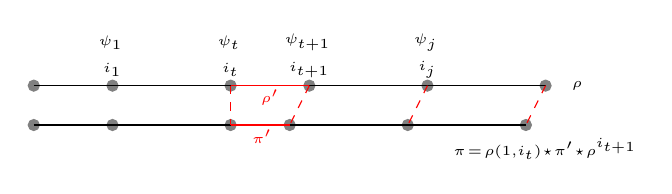
\begin{tikzpicture}
				%				[->,>=stealth',shorten >=1pt,auto,node distance=0,main node/.style={circle,draw}]
				\filldraw [gray] (0,0) circle (2pt)
				(1.0,0) circle (2pt)
				(2.5,0) circle (2pt)
				(3.5,0) circle (2pt) 
				(5.0,0) circle (2pt)
				(6.5,0) circle (2pt);
				%
				\filldraw [gray] (0,-0.5) circle (2pt)
				(1.0,-0.5) circle (2pt)
				(2.5,-0.5) circle (2pt)
				(3.25,-0.5) circle (2pt) 
				(4.75,-0.5) circle (2pt)
				(6.25,-0.5) circle (2pt);
				%
				\draw [red] (2.5,0) -- (3.5,0);
				\draw [black]  (0,0) -- (2.5,0);
				\draw [black] (3.5,0) -- (6.5,0);
				\draw [black] (0,-0.5) -- (2.5,-0.5);
				\draw [red] (2.5,-0.5) -- (3.25,-0.5);
				\draw [black] (3.25,-0.5) -- (6.25,-0.5);
				\draw [dashed, red] (2.5,0) -> (2.5,-0.5);
					\draw [dashed, red] (3.5,0) -> (3.25,-0.5);
				\draw [dashed, red] (5,0) -> (4.75,-0.5);
				\draw [dashed, red] (6.5,0) -> (6.25,-0.5);
				{\tiny
					\node (a0) at (6.9,0) {$\rho$};	
					\node (b0) at (6.5,-0.8) {$\pi\!=\!\rho(1,\! i_t)\!\star\! \pi'\! \star\! \rho^{i_{t+1}}$};	
					\node (a1) at (1,0.2) {$i_1$};
					\node (a2) at (2.5,0.2) {$i_t$};
					\node (a3) at (3.5,0.2) {$i_{t+1}$};
					\node (a4) at (5,0.2) {$i_{j}$};
					\node (a1) at (1,0.55) {$\hsE\! \psi_1$};
					\node (a2) at (2.5,0.55) {$\hsE\! \psi_{t}$};
					\node (a3) at (3.5,0.55) {$\hsE\! \psi_{t+1}$};
					\node (a4) at (5,0.55) {$\hsE\! \psi_{j}$};
					\node [red] (a4) at (2.9,-0.65) {$\pi'$};
					\node [red] (a4) at (3.0,-0.15) {$\rho'$};
				}
				
			\end{tikzpicture}}
	%\vspace{-0.5cm}
    \caption{Representation of the contraction step of Theorem~\ref{theorem:polynomialSizeModelProperty}---case $(i)$}\label{fig:contr2}
\end{figure}

Let us denote $\pi\star\sigma$ by $\overline{\pi}$ and $\rho\star\sigma$ by $\overline{\rho}$. Let $H:[1,|\overline{\pi}|] \rightarrow [1,|\overline{\rho}|]$ be the function mapping positions of $\overline{\pi}$ into positions of $\overline{\rho}$ in such a way that positions ``outside'' $\pi'$, i.e., outside the interval $[\alpha,\alpha+|\pi'|-1]$, are mapped into their original positions in $\overline{\rho}$ while those ``inside'' $\pi'$, i.e., in $[\alpha,\alpha+|\pi'|-1]$, are mapped into the corresponding positions in $\rho'$ (exploiting well-formedness of $\pi'$ w.r.t.\ $\rho'$):
%
\begin{equation*}
H(m) = \begin{cases}
	m& \text{if}\quad m<\alpha; \\
\alpha+\ell_{m-\alpha+1}-1 & \mbox{if}\quad \alpha\leq m<\alpha+|\pi'|; \\
m+(|\rho'| - |\pi'|) & \mbox{if}\quad m\geq \alpha+|\pi'|,
\end{cases}
\end{equation*}
where  $\ell_s$ is the $\rho'$-position corresponding to the $\pi'$-position $s$,
with $\ell_s\in\mathopen[1,|\rho'|\mathclose]$ and $s\in\mathopen[1,|\pi'|\mathclose]$.

It is easy to check that $H$ satisfies the following properties:
\begin{enumerate}
  \item $H$ is strictly monotonic, i.e., for all $j,j'\in [1,|\overline{\pi}|]$, $j<j'\iff H(j)<H(j')$;
  \item for all $j\in [1,|\overline{\pi}|]$, $\overline{\pi}(j)=\overline{\rho}(H(j))$;
  \item $H(1)= 1$ and $H(|\overline{\pi}|)=|\overline{\rho}|$;
  \item $Wt(\varphi,\overline{\rho})\subseteq \{H(j) \mid j \in [1,|\overline{\pi}|] \}$, i.e., all witness positions are preserved;
  \item for each $j\in [1,|\overline{\pi}|]$ and $p\in \Prop$, $\Ku,\overline{\pi}^{j}\models p\iff \Ku,\overline{\rho}^{H(j)}\models p$.
\end{enumerate}

The fact that
$\Ku,\overline{\pi}\models \varphi$ is an immediate consequence of the following claim, considering that  $H(1)=1$, $\Ku,\overline{\rho}\models \varphi$,  $\overline{\rho}^{1}=\overline{\rho}$, and $\overline{\pi}^{1}=\overline{\pi}$.

\begin{claim}  For all $j\in [1,|\overline{\pi}|]$, all subformulas $\psi$ of $\varphi$, and all $u\in\Trk_\Ku$, it holds that 
\[
\Ku,u\star \overline{\rho}^{H(j)}\models \psi \Longrightarrow \Ku,u\star\overline{\pi}^{j}\models \psi.
\]
\end{claim}
\begin{proof}
Assume that $\Ku,u\star\overline{\rho}^{H(j)}\models \psi $. Note that $u\star \overline{\rho}^{H(j)}$ is defined if and only if $u\star \overline{\pi}^{j}$ is defined. We prove by induction on the structure of $\psi$  that
$\Ku,u\star\overline{\pi}^{j}\models \psi$. Since $\varphi$ is in \nnf, only the following cases occur:
 \begin{itemize}
   \item $\psi= p$ or $\psi=\neg p$ for some $p\in \Prop$. By Property~5 of $H$, $\Ku, \overline{\pi}^{j}\models p$ if and only if $\Ku,\overline{\rho}^{H(j)}\models p$.
    Hence, $\Ku, u\star \overline{\pi}^{j}\models p$ if and only if $\Ku,u\star\overline{\rho}^{H(j)}\models p$, and the result holds.
    \item $\psi= \theta_1\wedge\theta_2$ or $\psi= \theta_1\vee\theta_2$, for some $\AAbarEEbar$ formulas $\theta_1$ and $\theta_2$: the result directly follows from the inductive hypothesis.
   \item $\psi = \hsEu\theta$. We need to show that for each proper suffix $\eta$ of $u\star\overline{\pi}^{j}$, $\Ku,\eta\models\theta$. We distinguish two cases:
 \begin{itemize}
   \item $\eta$ is \emph{not} a proper suffix of $\overline{\pi}^{j}$. Hence, $\eta$ is of the form $u^{h}\star \overline{\pi}^{j}$ for some $h\in [2,|u|]$. Since $\Ku,u\star\overline{\rho}^{H(j)}\models \hsEu\theta $, then
   $\Ku,u^{h}\star\overline{\rho}^{H(j)}\models \theta $.  By the inductive hypothesis, $\Ku,u^{h}\star\overline{\pi}^j\models \theta $.
   \item $\eta$ is a proper suffix of $\overline{\pi}^{j}$. Hence, $\eta = \overline{\pi}^{h}$ for some $h\in [j+1,|\overline{\pi}|]$.   By Property~1 of $H$, $H(h)>H(j)$, and since $\Ku,u\star\overline{\rho}^{H(j)}\models \hsEu\theta $, we have that $\Ku,\overline{\rho}^{H(h)}\models \theta $. By the inductive hypothesis,  $\Ku,\overline{\pi}^h\models \theta $.
 \end{itemize}
 Therefore, $\Ku,u\star \overline{\pi}^j\models \hsEu\theta $.
\item $\psi = \hsE\theta$. We need to show that there exists a proper suffix of $u\star\overline{\pi}^{j}$ satisfying $\theta$. %Since $\Ku,\overline{\pi}^{h}\models\theta$.
Since $\Ku,u\star \overline{\rho}^{H(j)}\models \psi $, there exists a proper suffix $\eta'$ of  $u\star \overline{\rho}^{H(j)}$
 such that  $\Ku,\eta'\models \theta $. We distinguish two cases:
 \begin{itemize}
   \item $\eta'$ is \emph{not} a proper suffix of $\overline{\rho}^{H(j)}$. Hence, $\eta'$ is of the form $u^{h}\star \overline{\rho}^{H(j)}$ for some $h\in [2,|u|]$. By the inductive hypothesis, $\Ku,u^{h}\star\overline{\pi}^j\models \theta $. Hence, $\Ku,u\star\overline{\pi}^j\models \hsE\theta $.
   \item $\eta'$ is a proper suffix of $\overline{\rho}^{H(j)}$. Hence, $\eta' = \overline{\rho}^{i}$ for some $i\in [H(j)+1,|\overline{\rho}|]$, and $\Ku,\overline{\rho}^{i}\models \theta $.
   Let $i'$ be the greatest position of $\overline{\rho}$ such that $\Ku,\overline{\rho}^{i'}\models\theta$. Hence $i'\geq i$ and, by Definition~\ref{definition:WitnessPositions}, $i'\in Wt(\varphi,\overline{\rho})$. By Property 4 of $H$, $i'=H(h)$ for some $\overline{\pi}$-position $h$. Since $H(h)>H(j)$, it holds that $h>j$ (Property 1). By the inductive hypothesis, $\Ku,\overline{\pi}^h\models \theta $, and we obtain that $\Ku,u\star\overline{\pi}^j\models \hsE\theta $.
 \end{itemize}
  Therefore, in both the cases, $\Ku,u\star \overline{\pi}^j\models \hsE\theta $.
 \item $\psi=\hsEtu\theta$ or $\psi=\hsEt\theta$: the thesis holds as a direct consequence of the inductive hypothesis.
 \item $\psi = \hsAu\theta$, $\psi=\hsA\theta$, $\psi = \hsAtu\theta$, or $\psi=\hsAt\theta$. Since $u\star\overline{\pi}^j$ and $u\star\overline{\rho}^{H(j)}$ start at the same state and lead to the same state (by Properties 2 and 3 of $H$), the thesis trivially follows. This concludes the proof of the claim.\qedhere
\end{itemize}
\end{proof}
%
We have shown that $\Ku,\overline{\pi}\models \varphi$, with $|\pi| < |\rho |$. Now, if $|\pi|\leq |\States| \cdot (|\varphi|+1)^2$, the thesis is proved; otherwise, the above contraction step can be iterated a finite number of times, until the bound is reached, proving the thesis of Theorem~\ref{theorem:polynomialSizeModelProperty}.
  \end{proof}
  
\subsection{\PSPACE\ MC algorithm for $\AAbarEEbar$}\label{subsec:MCpolyAAbarEEbar}

By exploiting the polynomial small-model property stated by Theorem~\ref{theorem:polynomialSizeModelProperty}, it is easy to define a \PSPACE\ MC algorithm for $\AAbarEEbar$. The main MC procedure for $\AAbarEEbar$ formulas is \texttt{ModCheck}$(\Ku,\psi)$ (Algorithm~\ref{ModCheck2}). All the initial traces $\sigma$, obtained by visiting the unravelling of $\Ku$ from its initial state $\sinit$ up to depth $|\States|\cdot (2|\psi|+3)^2$, are checked with respect to $\psi$ by the function
$\texttt{Check}(\Ku, \psi,\sigma)$ (Algorithm~\ref{Chk2}) which decides whether $\Ku,\sigma\models \psi$. The $\texttt{Check}$ function is iteratively called until either some initial trace is found that does not satisfy $\psi$ or all bounded initial traces satisfy $\psi$ (and thus $\Ku\models\psi$). The invocation of $\texttt{Check}(\Ku, \psi,\sigma)$ (Algorithm~\ref{Chk2}) decides whether $\Ku,\sigma\models \psi$ or not by recursively calling itself on the subformulas  of $\psi$ either over $\sigma$ or over (bounded) traces obtained by unraveling $\Ku$ forward (starting from $\lst(\sigma)$) for occurrences of the modality  $\hsA$,  and backward  (starting from $\fst(\sigma)$) for occurrences of $\hsAt$ and
$\hsEt$.

\begin{algorithm}[p]
\begin{algorithmic}[1]
	\For{all initial traces $\sigma\in\Trk_\Ku$ such that $|\sigma|\leq |\States|\cdot (2|\psi|+3)^2$}
	    \If{$\texttt{Check}(\Ku,\psi,\sigma)=0$}
	        \Return{0: ``$\Ku,\sigma\not\models \psi$''}\Comment{Counterexample found}
	    \EndIf
	\EndFor
	\Return{1: ``$\Ku\models \psi$''}%\Comment{Counterexample not found}	
\end{algorithmic}
\caption{\texttt{ModCheck}$(\Ku,\psi)$}\label{ModCheck2}
\end{algorithm}


\begin{algorithm}[p]
\begin{algorithmic}[1]
    \If{$\psi=p$, for $p\in\Prop$}%\Comment{$\psi=\neg p$ is similar}
	    \If{$p\in \bigcap_{s\in \states(\sigma)}\mu(s)$}
	        \State{\textbf{return} 1 \textbf{else} \textbf{return} 0}
	    \EndIf
	\ElsIf{$\psi=\neg\varphi$}
        \Return{$1-\texttt{Check}(\Ku,\varphi,\sigma)$}
    \ElsIf{$\psi=\varphi_1\wedge\varphi_2$}%\Comment{$\psi=\varphi_1\vee\varphi_2$ similar}
        \If{$\texttt{Check}(\Ku,\varphi_1,\sigma)=0$}
	        \Return{0}
	    \Else
	        \Return{$\texttt{Check}(\Ku,\varphi_2,\sigma)$}
	    \EndIf
	\ElsIf{$\psi=\hsA\varphi$}%\Comment{$\psi=\hsAt\varphi$ is similar}
	    \For{all $\pi\in\Trk_\Ku$ such that $\fst(\pi)=\lst(\sigma)$, and $|\pi|\leq |\States|\cdot (2|\varphi|+1)^2$}
	        \If{$\texttt{Check}(\Ku,\varphi,\pi)=1$}
	            \Return{1}
	        \EndIf
	    \EndFor
	    \Return{0}
%\columnbreak %%%%%%%%%%%%%%%%%%%%%%%%%%%%%%%%%%%%%%%%%%%%%%%%%%%%%%%%%%%%%%%%%%%%%%%%%%%%%%%%%%%%%%%	
	\ElsIf{$\psi=\hsE\varphi$}%\Comment{$\psi=[E]\varphi$ is similar}
	    \For{each proper suffix $\pi$ of $\sigma$}
	        \If{$\texttt{Check}(\Ku,\varphi,\pi)=1$}
	            \Return{1}
	        \EndIf
	    \EndFor
	    \Return{0}
	\ElsIf{$\psi=\hsEt\varphi$}
        \For{all $\pi\in\Trk_\Ku$ such that $\lst(\pi)=\fst(\sigma)$, and $2\leq |\pi|\leq |\States|\cdot (2|\varphi|+1)^2$}
            \If{$\texttt{Check}(\Ku,\varphi,\pi\star\sigma)=1$}
                \Return{1}
            \EndIf
        \EndFor
	    \Return{0}
	\EndIf
	\State{\dots}\Comment{$\psi=\hsAt\varphi$ is analogous to $\psi=\hsA\varphi$}
\end{algorithmic}
\caption{\texttt{Check}$(\Ku,\psi,\sigma)$}\label{Chk2}
\end{algorithm}

Note that the considered bound on the length of initial traces is actually  $|\States|\cdot (2|\psi|+3)^2\geq |\States|\cdot (|\nnf(\neg\psi)|+1)^2$ (line 1 of the \texttt{ModCheck} procedure).
The reason is that the correctness proof of the algorithm exploits the polynomial bound of Theorem~\ref{theorem:polynomialSizeModelProperty} over the formula $\neg\psi$, that has to be converted into \nnf .

%by basically calling itself recursively on the sub-formulas of $\psi$ and unravelling again $\Ku$---
%Note that the for-loop at the first line considers all initial traces having length at most $|W|\cdot (2|\psi|+3)^2\geq |W|\cdot (|\nnf(\neg\psi)|+1)^2$. 


The next results state soundness and completeness of  Algorithm~\ref{Chk2} and Algorithm~\ref{ModCheck2}, respectively. Their proofs can be found in Appendix~\ref{proof:lemmamdc} and \ref{proof:ThCorrComplMC}.

\begin{lemma}\label{lemmamdc}
Let $\psi$ be an $\AAbarEEbar$ formula, $\Ku$ be a finite Kripke structure, and $\sigma\in\Trk_\Ku$. Then, $\texttt{Check}(\Ku, \psi,\sigma)=1$ if and only if $\Ku,\sigma\models \psi$.
\end{lemma}

\begin{theorem}\label{ThCorrComplMC}
Let $\psi$ be an $\AAbarEEbar$ formula and $\Ku$ be a finite Kripke structure. Then, \texttt{ModCheck}$(\Ku,\psi)=1$ if and only if $\Ku\models \psi$.
\end{theorem}


The MC procedures require \emph{polynomial working space}, since:
\begin{itemize}
        \item \texttt{ModCheck} needs to store only a trace no longer than $|\States|\cdot (2|\psi|+3)^2$ (obviously, many traces are generated while visiting the unravelling of $\Ku$, but only one at a time needs to be stored);
        \item every recursive call to \texttt{Check} (possibly) needs space for a trace no longer than $|\States|\cdot
        (2|\varphi|+1)^2$, where $\varphi$ is a subformula of $\psi$ such that $|\varphi|\leq |\psi|-1$;
        \item at most one call to \texttt{ModCheck} and $|\psi|$ calls to \texttt{Check} can be simultaneously active.
\end{itemize}
Thus the maximum space needed by the given algorithms is $(|\psi|+1)\cdot O(\log |\States|)\cdot (|\States|\cdot (2|\psi|+3)^2)$ bits, where $O(\log |\States|)$ bits are needed to represent a state of $\Ku$. 

Theorem~\ref{ThCorrComplMC}, along with the above space analysis and the fact that
MC for the fragment $\Ebar$ is \PSPACE-hard (see Appendix~\ref{sect:BbarHard}), entail the following corollary.
%
\begin{corollary}
The MC problem for $\AAbarEEbar$ formulas over finite Kripke structures is \PSPACE-complete.
\end{corollary}
%
The same result, that is, \PSPACE-completeness, clearly holds also for any sub-fragment of $\AAbarEEbar$ which features modality $\Ebar$. %In the following we consider the small fragments $\B$ and $\E$.


\subsection{$\co\NP$ MC algorithm for $\B$ and $\E$}\label{sec:TheFragmentE}
We now conclude the section by showing that the MC problem for the  fragments $\B$ and $\E$ is in $\co\NP$, that is, they have the same complexity as the purely propositional fragment $\HSprop$ (proved to be hard for $\co\NP$ in~\cite{MMP15B}). We focus on $\E$, as the case  of  $\B$ is completely symmetric. As we will see, the MC algorithm heavily rests again on the polynomial small-model property. 

\begin{algorithm}[tp]
\begin{algorithmic}[1]
	\State{$\rho\gets \texttt{A\_trace}(\Ku,\sinit,|\psi|)$}\Comment{a trace of $\Ku$ from $\sinit$ of length $\leq |\States|\cdot (2|\psi|+3)^2$}
	\If{$\texttt{CheckE}(\Ku,\psi,\rho)=\bot$}
	    \Return{\textbf{Yes}: ``$\Ku,\rho\not\models \psi$''}\Comment{Counterexample found}
	\Else
	    \Return{\textbf{No}: ``$\Ku,\rho\models \psi$''}\Comment{Counterexample \emph{not} found}	
	\EndIf
\end{algorithmic}
\caption{\texttt{CounterExE}$(\Ku,\psi)$}\label{ModCheckE}
\end{algorithm}


\begin{algorithm}[tp]
\begin{algorithmic}[1]
\State{$T\gets \texttt{New\_Bool\_Table}(|\psi|,|\rho|)$}\Comment{creates new table of $|\psi|\cdot |\rho|$ Boolean entries}
\For{all subformulas $\varphi$ of $\psi$ by increasing length}
    \If{$\varphi=p$, for $p\in\Prop$}
        \State{$T[p,|\rho|]\gets p\in \mu(\lst(\rho))$}
        \For{$i=|\rho|-1,\ldots ,1$}
            \State{$T[p,i]\gets T[p,i+1]$ and $p\in \mu(\rho(i))$}
        \EndFor
	\ElsIf{$\varphi=\neg \varphi_1$}
	    \For{$i=|\rho|,\ldots ,1$}
            \State{$T[\varphi,i]\gets$ not $T[\varphi_1,i]$}
        \EndFor

%\columnbreak %%%%%%%%%%%%%%%%%%%%%%%%%%%%%%%%%%%%%%%%%%%%%%%%%%%%%%%%%%%%%%%%%%%%%%%%%%%%%%%%%%%%%%%

    \ElsIf{$\varphi=\varphi_1\wedge\varphi_2$}
        \For{$i=|\rho|,\ldots ,1$}
            \State{$T[\varphi,i]\gets T[\varphi_1,i]$ and $T[\varphi_2,i]$}
        \EndFor
	\ElsIf{$\varphi=\hsE\varphi_1$}
	    \State{$T[\varphi,|\rho|]\gets\bot$}
	    \For{$i=|\rho|-1,\ldots ,1$}
            \State{$T[\varphi,i]\gets T[\varphi,i+1]$ or $T[\varphi_1,i+1]$}
	    \EndFor
	\EndIf
\EndFor	
\Return{$T[\psi,1]$}
\end{algorithmic}
\caption{\texttt{CheckE}$(\Ku,\psi,\rho)$}\label{ChkE}
\end{algorithm}

The algorithm is based on the \emph{non-deterministic} procedure
\texttt{CounterExE}$(\Ku,\psi)$  (Algorithm~\ref{ModCheckE}) which searches for counterexamples to the input $\E$ formula $\psi$ (that is, initial traces satisfying $\neg\psi$). If such a counterexample is found, clearly $\Ku\not\models \psi$. First, the procedure generates in a \emph{non-deterministic way} an initial trace $\rho$, whose length is at most $|\States|\cdot (2|\psi|+3)^2$, by means of $\texttt{A\_trace}(\Ku,\sinit,|\psi|)$. 
Then, the \emph{deterministic} function $\texttt{CheckE}(\Ku,\psi,\rho)$,  reported in Algorithm~\ref{ChkE}, evaluates $\psi$ over $\rho$. If \texttt{CheckE} returns $\bot$, a counterexample has been found and \texttt{CounterExE} returns \textbf{Yes} (thus the non-deterministic computation of the algorithm is successful). 
Otherwise, it returns \textbf{No} (the computation fails). 

As for the function \texttt{CheckE}, the following result holds. 
\begin{proposition} Let  $\psi$ be an $\E$ formula, $\Ku$ be a finite Kripke structure, and $\rho$ be a trace of $\Ku$. Then,
    \texttt{CheckE}$(\Ku,\psi,\rho)=\top $ if and only if $\Ku,\rho\models\psi$. 
\end{proposition}
\texttt{CheckE} exploits a Boolean
table $T$ with an entry for each pair consisting of a subformula of $\psi$ and the starting position of a suffix of $\rho$ (the size of $T$ is then $|\psi| \cdot |\rho|$). The function scans all the subformulas $\varphi$ of the input $\psi$ by increasing length, and it stores in the Boolean entry $T[\varphi,i]$, for $1\leq i\leq |\rho|$, whether $\Ku,\rho^i\models \varphi$ or not. 
Note that the result of the evaluation of $\psi$ over $\rho$ is stored in $T[\psi,1]$, as $\rho^1=\rho$.
Since subformulas of $\psi$ are considered by increasing length order, during an iteration starting at line 2,  when a subformula $\varphi$ of $\psi$ is being processed, it holds that $T[\xi,i]$ is defined for all other subformulas $\xi$ processed in some previous iteration, and $T[\xi,i]\!=\!\top$ iff $\Ku,\rho^i\!\models\! \xi$. Hence, at the end,
$T[\psi,1]\!=\!\top$ iff $\Ku,\rho \!\models\! \psi$.

We can now prove that the procedure \texttt{CounterExE} is sound and complete.
If \texttt{CounterExE}$(\Ku,\psi)$ has a successful computation, then there exists an initial trace $\rho$ such that $\texttt{CheckE}(\Ku,\psi,\rho)=\bot$. This means that $\Ku,\rho\not\models\psi$, and thus $\Ku\not\models\psi$.
%
Conversely, if $\Ku\not\models\psi$ then there exists an initial trace $\rho$ such that $\Ku,\rho\not\models \psi$.
By Theorem~\ref{theorem:polynomialSizeModelProperty}, there exists an initial trace $\pi$, whose length is bounded by $|\States|\cdot (|\psi'|+1)^2\leq |\States|\cdot (2|\psi|+3)^2$, such that $\Ku,\pi\models \psi'$, where $\psi'$ is the \nnf{} of $\neg\psi$.
Now, some non-deterministic instance of $\texttt{A\_trace}(\Ku,\sinit,|\psi|)$ generates exactly such $\pi$, being $|\pi|\leq |\States|\cdot (2|\psi|+3)^2$. Moreover, $\texttt{CheckE}(\Ku,\psi,\pi)=\bot$, and thus
\texttt{CounterExE}$(\Ku,\psi)$ has a successful computation.

\texttt{CounterExE}$(\Ku,\psi)$ is in $\NP$, as the generated trace(s) $\rho$ has (have) a length polynomial in $|\States|$ and $|\psi|$, and can thus be computed in polynomial time. Moreover, \texttt{CheckE} performs a polynomial number of steps, since all it has to do is filling in the table $T$, which features $|\psi|\cdot |\rho|$ entries.

\begin{corollary}\label{cor:E}
The MC problem for $\E$ formulas over finite Kripke structures is $\co\NP$-complete.
\end{corollary}
\begin{proof}
Since \texttt{CounterExE}$(\Ku,\psi)$ has a successful computation if and only if $\Ku\not\models \psi$, and such a procedure runs in (non-deterministic) polynomial time, the MC problem belongs to $\co\NP$. 
%
The $\co\NP$-hardness derives immediately from that of the purely propositional $\HS$ fragment $\HSprop$, as proved in~\cite{MMP15B}.
\end{proof}

In the next section we will see what happens if we add $\Bbar$ to $\AAbarEEbar$, and $\Ebar$ to $\AAbarBBbar$: we shall prove a different (this time, exponential) small-model property for $\AAbarEBbarEbar$ and $\AAbarBBbarEbar$, which will allow us to devise an $\EXPSPACE$ MC algorithm for them.